\documentclass{article}

% NeurIPS 2024 Style Package
\usepackage[final]{neurips_data_2024} % Use 'final' for camera-ready version
\usepackage[utf8]{inputenc} % allow utf-8 input
\usepackage[T1]{fontenc}    % use 8-bit T1 fonts
\usepackage{hyperref}       % hyperlinks
\usepackage{url}            % simple URL typesetting
\usepackage{booktabs}       % professional-quality tables
\usepackage{amsfonts}       % blackboard math symbols
\usepackage{nicefrac}       % compact symbols for 1/2, etc.
\usepackage{microtype}      % microtypography
\usepackage{graphicx}       % for including images
\usepackage{caption}        % for figure captions
\usepackage{subcaption}     % for subfigures
\usepackage{amsmath}        % for math equations
\usepackage{cleveref}       % for smart cross-referencing
\usepackage{float}         % in your preamble


\title{COMS4060A/7056A --- Assignment 1: Analysis of Vehicle Fueling Data}

\author{%
  Mayuri Balakistan \\
  Student Number: 2543986\\
  Department of Computer Science\\
  Wits University\\
  \texttt{2543986@student.wits.ac.za} \\
  % examples of more authors
  % \And
  % Coauthor \\
  % Affiliation \\
  % Address \\
  % \texttt{email} \\
  % \AND
  % Coauthor \\
  % Affiliation \\
  % Address \\
  % \texttt{email} \\
  \And
  Taboka Chloe Dube \\
  Student Number: 2602515\\
  Department of Computer Science \\
  Wits University \\
\texttt{2602515@student.wits.ac.za} \\
  \And
  Wendy Maboa \\
  Student Number: 2541693\\
  Department of Computer Science \\
  Wits University \\
\texttt{2541693@student.wits.ac.za} \\
}
\begin{document}

\maketitle

\begin{abstract}
This report details the process of cleaning, feature engineering, and analyzing a global dataset of vehicle fuel transactions. The raw data contained inconsistencies in date formats, numeric fields, and currency representations. We applied multiple data cleaning protocols, including regex validation, outlier removal, and unit conversion. New features were engineered to extract user, vehicle, and currency information, and to standardize measurements into the metric system. The cleaned dataset was subsequently analyzed to explore trends in user demographics, vehicle age and popularity, and fuel consumption patterns across different countries. 
\end{abstract}

\section{Introduction}
 This project analyzes a dataset containing records of vehicle fuel purchases from users around the world. The initial dataset was messy, containing mixed date formats, missing values, inconsistent numeric entries, and currency symbols embedded within numeric cost fields. This report outlines the comprehensive data cleaning pipeline developed to handle these issues, the feature engineering steps taken to enrich the dataset, and the subsequent exploratory data analysis performed to extract insights into global vehicle usage patterns.

\section{Data Cleaning}

\subsection{Date Fields}
The initial date format was \textbf{DD mmm YYYY}. To assess data quality, a regex mask was created to identify entries conforming to this format.
\begin{enumerate}
    \item The proportion of entries in the \texttt{date\_fueled} column not matching this format was found to be \textbf{11.68\%}.
    \item Invalid \texttt{date\_fueled} entries were replaced with valid \texttt{date\_captured} values where possible.
    \item Valid entries were converted to a standardized \textbf{YYYY-MM-DD} format using \texttt{pd.to\_datetime}, with invalid years (outside 1900--2099) set to \texttt{NaT}.
    \item Date fields were clamped to a plausible range (1 January 2025 to 1 September 2025 - the date on which this question was done) to remove extreme outliers.
    \item Plotting the distribution of fueling dates as a histogram, shows that years post 2005, had an increasing number of fueled cars, there is a significant drop in 2020 which can be attributed to COVID-19 quarantine regulations ,then post covid, number of fueled cars increases again, which can be attributed again to relaxation of quarantine rules and potentially people buying more cars. Further, the highest most recent fueling dates are up to 2022.

    \begin{figure}[htbp]
    \centering
    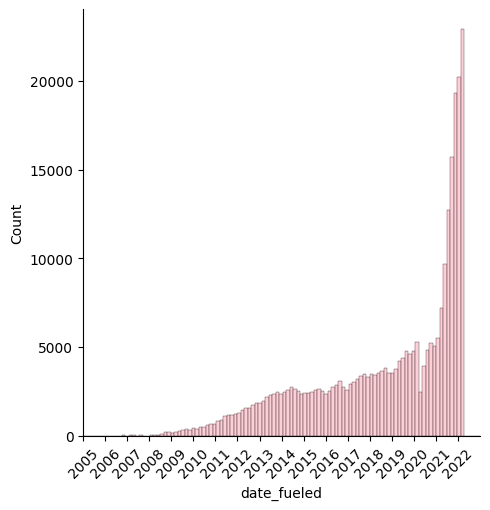
\includegraphics[width=0.6\textwidth]{images/fueled_dates_histo.png}
    \caption{Distribution of vehicle fueling dates. A significant drop in 2020 is attributed to COVID-19 quarantine regulations, followed by a recovery as restrictions were lifted.}
    \label{fig:fuel_dates}
\end{figure}
 
\end{enumerate}


\subsection{Numeric Fields}
The numeric fields \texttt{gallons}, \texttt{miles}, and \texttt{mpg} were cleaned as follows:
\begin{enumerate}
    \item To find these percentages, a null count for each was found and then calculated against the size of the dataframe at that point and multiplied by 100. The method \texttt{.isnull()} accounts for NaNs, None and Null values.
    \item  First, the rows in which 2 or more of these values were missing were dropped as these would not provide useful information. MPG can be calculated as $MPG = \frac{miles}{gallons}$. $Gallons = \frac{miles}{mpg}$ and Miles = gallons * mpg, in the notebook, this was done after number 3, which is converting the respective values to floats. This is because the code would struggle to compute the missing values using strings and floats combined as opposed to standardized.

    \item  To convert these values to floats, considerations for the commas and periods had to be made. To account for these, the \textbf{str.replace(‘,’, ‘ ’)} function was used. Then they would be cast to be of type float using \textbf{astype(float)}.
    \item The MPG distribution is right-skewed: most vehicles cluster around lower MPG values, but there’s a tail extending to higher efficiencies. This could mean alot of cars in this data set consume alot of fuel per mile.The miles distribution is strongly right-skewed, suggesting that most trips are relatively short, with the highest concentration between 0–10,000 miles. There are smaller occurrences approximately 20,000, 30,000, and 50,000 miles, representing occasional longer trips. Overall, the distribution suggests that short trips dominate the dataset, while high-mileage trips are rare.The gallons distribution is right-skewed, with most fuel purchases concentrated at the lower end of the range (0–2,500 gallons). Very few extremely large values appear beyond 15,000 gallons, creating a large gap in the distribution. This indicates that most people fill up fuel in the 0-2500 range, while a very large fill is likely a recording error or a large vehicle such as a truck.

    This can be viewed in the image below:

    \begin{figure}[htbp]
    \centering
    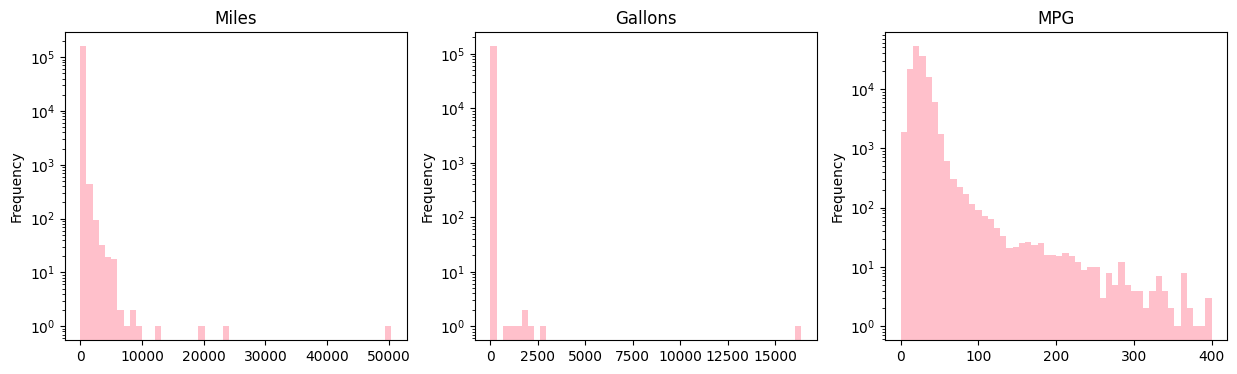
\includegraphics[width=0.6\textwidth]{images/numeric_distributions.png}
    \caption{Distribution of MPG, Miles and Gallons. Showing the skewness.}
    \label{fig:fuel_dates}

\end{figure}

 \item The statistical distributions of the cleaned numerical fields were computed. At this stage, the dataframe had been significantly processed, resulting in feasible value ranges for the \texttt{date\_fueled}, \texttt{date\_captured}, \texttt{gallons}, \texttt{mpg}, and \texttt{miles} columns. A notable anomaly was observed: the maximum value for the \texttt{date\_fueled} field was `2024-12-07', while the maximum \texttt{date\_captured} was `2022-04-16'. This discrepancy indicates that some \texttt{date\_fueled} entries are likely bogus, as they refer to dates in the future relative to their capture date.

    
\end{enumerate}


\section*{Question 2: Feature Engineering}

\subsection*{Currency Extraction}
The \texttt{total\_spent} and \texttt{cost\_per\_gallon} columns originally included both numeric values and currency symbols (e.g., R500, \$70). We extracted the currency symbols into a new column, \texttt{currency}, and cleaned the numeric parts into proper floats. This allowed for easier comparison of costs across different countries while still retaining the currency as a categorical variable.

\subsection*{Float Values for Costs}
After separating the currency symbols, both \texttt{total\_spent} and \texttt{cost\_per\_gallon} were converted into numeric columns. This was essential for calculations such as average prices, comparisons across time, and further statistical analysis.

\subsection*{User and Vehicle Information}
The user ID, car make, model, and year were extracted from the \texttt{user\_url} field. The last part of the URL was used as the user ID, while other segments provided the car details. This enriched the dataset by linking fuel transactions to individual users and specific vehicles.

\subsection*{Metric System Conversion}
Since the dataset was in imperial units, I converted the values into metric units, which are more standard in South Africa:
\begin{itemize}
    \item Litres Filled: Computed from gallons (1 US gallon $\approx$ 3.785 litres).
    \item Kilometres Driven: Converted from miles (1 mile $\approx$ 1.609 km).
    \item Litres per 100km: Derived as $(\texttt{litres} / \texttt{km\_driven}) * 100$. This metric is a widely used standard to measure fuel efficiency.
\end{itemize}

\subsection*{Discussion}
These new features added greater interpretability and standardisation to the dataset. For example, litres per 100km allows us to compare vehicle efficiency in a way that is familiar and directly meaningful to local contexts, while extracting user and vehicle details enabled us to later perform country- and vehicle-specific analyses.


\section{Vehicle Exploration}

\subsection{Unique Users per Country}
Countries were proxied by their currency. \Cref{fig:users_per_country} shows that developed nations (e.g., USA, UK) have the largest user bases, while developing countries have the smallest, likely reflecting higher rates of personal vehicle ownership and app adoption in wealthier nations.

\begin{figure}[htbp]
    \centering
    \includegraphics[width=0.9\textwidth]{}
    \caption{Number of unique users per country, proxied by currency.}
    \label{fig:users_per_country}
\end{figure}

\subsection{App Popularity Over Time}
\Cref{fig:users_per_day} plots the number of unique users per day. The sharp increase in the 2010s and early 2020s correlates with the widespread adoption of smartphones and apps. The decline after 2022 is likely an artifact of data collection ending rather than a drop in actual popularity.

\begin{figure}[htbp]
    \centering
    \includegraphics[width=0.9\textwidth]{media/image5.png}
    \caption{Number of unique users per day, showing the app's growth over time.}
    \label{fig:users_per_day}
\end{figure}

\subsection{Vehicle Age Distribution by Country}
\Cref{fig:vehicle_age} shows the distribution of vehicle ages (based on fueling date) for the top 20 countries. Most vehicles globally are less than 20 years old, with a median age of approximately 10 years.

\begin{figure}[htbp]
    \centering
    \includegraphics[width=0.9\textwidth]{media/image4.png}
    \caption{Distribution of vehicle age per country.}
    \label{fig:vehicle_age}
\end{figure}

\subsection{Popular Vehicle Makes and Models}
The most popular car makes are Toyota, Ford, and BMW. The most popular models are the Civic, Jetta, and Land Cruiser (\Cref{fig:pop_models}).

\begin{figure}[htbp]
    \centering
    \begin{subfigure}[b]{0.45\textwidth}
        \centering
        \includegraphics[width=\textwidth]{media/image3.png}
        \caption{Popular car makes.}
    \end{subfigure}
    \hfill
    \begin{subfigure}[b]{0.45\textwidth}
        \centering
        \includegraphics[width=\textwidth]{media/image1.png}
        \caption{Popular car models.}
    \end{subfigure}
    \caption{Popularity of vehicle makes and models.}
    \label{fig:pop_models}
\end{figure}


\section{Fuel Usage}
\subsection{Outlier Removal}
For meaningful analysis, outliers were removed for the top five currencies (\$, £, CA\$, €, R).

\begin{enumerate}
    \item The top currencies were identified by computing the frequency count of each currency symbol and sorting these counts in descending order. The five most frequent currencies, corresponding to the United States (US\$), United Kingdom (£), Canada (CA\$), the Eurozone (€), and South Africa (R), were selected for subsequent analysis.

    \item To ensure a meaningful and comparable analysis across these economic regions, we implemented a currency-specific outlier removal protocol. For each of the top five currencies, we calculated the 1st and 99th percentiles for the variables \texttt{total\_spent}, \texttt{gallons}, \texttt{cost\_per\_gallon}, \texttt{miles}, and \texttt{mpg}. These percentiles were used to define upper and lower bounds for plausible values, which were tailored to each currency to account for differences in fuel prices and consumption habits. All rows containing values outside these designated thresholds for their respective currency were removed. This process refined the dataset by eliminating extreme and implausible entries, which reduced the total count of observations, adjusted summary statistics like the mean, and narrowed the value ranges to more representative distributions.

    \item Following the definition of these realistic thresholds, they were applied to filter the dataset. This critical cleaning step was performed to achieve three objectives:
    \begin{itemize}
        \item Eliminate outliers that could skew statistical analyses and visualizations.
        \item Ensure comparability across different currencies by controlling for regional economic factors.
    \end{itemize}
\end{enumerate}

\section*{Section 4.3: Fuel Usage In South Africa}

\subsection*{Filtering South African Data}
The dataset was filtered to include only records where the currency was Rand (R). This gave us a clean subset (\texttt{sa\_df}) representing South African users, but some SA users incorrectly logged in USD, meaning our dataset may undercount South African drivers.

\subsection*{Fuel Prices Over Time}
The \texttt{cost\_per\_gallon} column was cleaned to numeric form, and fuel prices were plotted over time. This provided a general view of how fuel prices in SA fluctuated across the dataset, showing periods of increases and decreases, but over time, they gradually increased.

\begin{figure}[H]
    \centering
    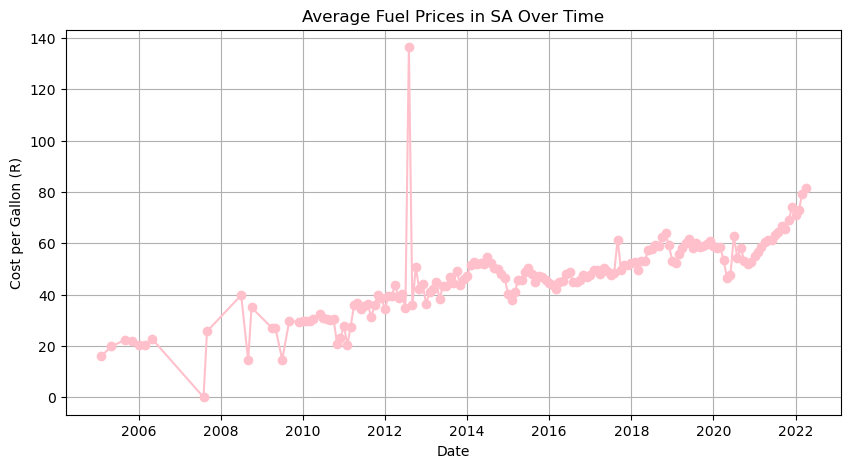
\includegraphics[width=0.8\textwidth]{images/Average Fuel Prices.png}
    \caption{Fuel Prices Over Time in South Africa}
\end{figure}


\subsection*{Refueling by Day of Week}
A bar chart of fueling activity by weekday was produced. This revealed overall patterns of consumer behavior during the week, with particular interest in the fact that Tuesdays had higher refueling rates compared to other days.

\begin{figure}[h]
    \centering
    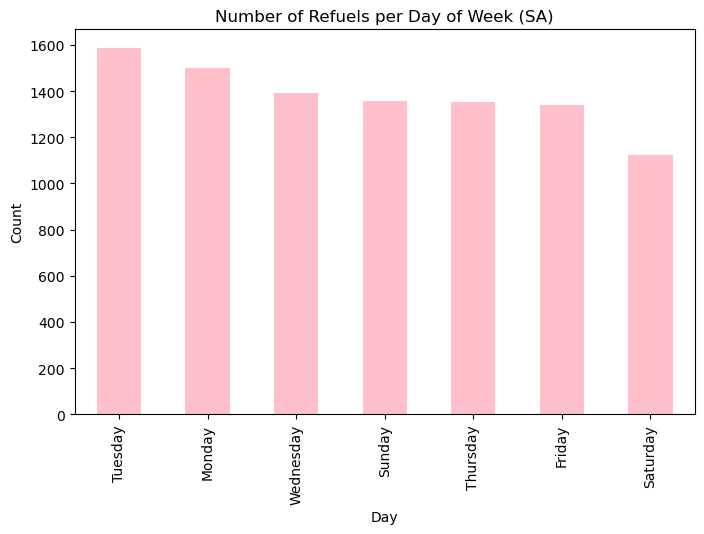
\includegraphics[width=0.7\textwidth]{images/Number of refuels.png}
    \caption{Refueling Activity by Day of Week}
\end{figure}

\subsection*{First Tuesdays vs First Wednesday Analysis}
The dataset was further restricted to only the first Tuesday and Wednesday of each month. This was crucial for examining the direct impact of price adjustments, since fuel prices are reset on the first Tuesday of the month in South Africa.

\subsection*{Price Change Indicator}
A \texttt{price\_change} column was created to indicate whether the price went up or down after the adjustment. This allowed grouping and comparison of consumer behavior based on the direction of the price change. And it was noticed that the \texttt{price\_trend} for the first Tuesday (row1), Wednesday (row2), Wednesday (row3), and Tuesday (row4) went up.

\begin{figure}[h]
    \centering
    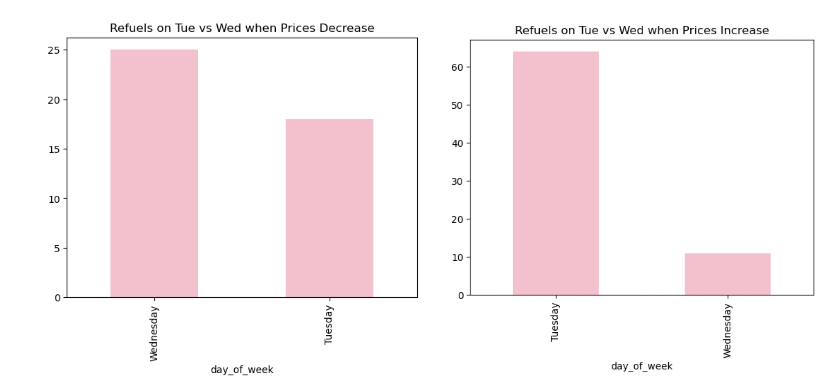
\includegraphics[width=0.9\textwidth]{images/Screenshot 2025-09-07 222047.png}
    \caption{Consumer Refueling Behavior Based on Price Change}
\end{figure}

\subsection*{Findings}
When prices decreased, more users tended to refuel on Wednesday, postponing their purchase to take advantage of the lower cost.

When prices increased, more users tended to refuel on Tuesday, anticipating the rise and filling up before the higher price took effect.

\subsection*{Discussion}
These findings align with economic intuition: consumers strategically time their refueling around predictable price changes to minimize costs. The plots clearly illustrated this behavior, showing noticeable shifts between Tuesday and Wednesday refueling counts depending on whether prices were going up or down.

\section{Conclusion}
This project successfully transformed a raw, inconsistent dataset into a clean, enriched resource for analysis. Through methodical data cleaning and insightful feature engineering, we were able to standardize the data and uncover significant trends. Key findings include the correlation between economic development and app usage, the relative youth of vehicle fleets in top user countries, and the market dominance of specific automotive brands. The methodologies developed here provide a robust framework for handling similar real-world datasets in the future.

\end{document}